
%%%%%%%%%%%%%%%%%%%%%%%%%%%%%%%%%%%%%%%%%%%%%%%%%%%%%%%%%%%%%%%%%%%%%%%%%%%%%%%%
%%                                                                
%%      SWSC LaTeX class for Journal of Space Weather and Space Climate
%%      
%%                                      (c) Springer-Verlag HD
%%                                      revised by EDP Sciences
%%                                      further revised by J. Watermann 
%%
%%%%%%%%%%%%%%%%%%%%%%%%%%%%%%%%%%%%%%%%%%%%%%%%%%%%%%%%%%%%%%%%%%%%%%%%%%%%%%%%
%%
%%      This demonstration file was derived from aa.dem
%%  
%%      AA vers. 7.0, LaTeX class for Astronomy & Astrophysics
%%      demonstration file
%%                                                (c) Springer-Verlag HD
%%                                                revised by EDP Sciences
%%
%%%%%%%%%%%%%%%%%%%%%%%%%%%%%%%%%%%%%%%%%%%%%%%%%%%%%%%%%%%%%%%%%%%%%%%%%%%%%%%%
%%
%%      modified for Journal of Space Weather and Space Climate
%%      by Jurgen Watermann, Editorial Advisor to SWSC
%%
%%      01-04-2012
%%      02-04-2012 revision 1
%%      12-07-2012 revision 2
%%      06-12-2012 revision 3 
%%      01-01-2014 revision 4
%%      06-03-2014 revision 4.1
%%
%%%%%%%%%%%%%%%%%%%%%%%%%%%%%%%%%%%%%%%%%%%%%%%%%%%%%%%%%%%%%%%%%%%%%%%%%%%%%%%%
%%
%%      The two sub-figures referenced in this template are of eps and png type,
%%      respectively, in order to demonstrate the usepackages subfigure and
%%      epstopdf and thus create pdf-only output 
%%
%%      If you want to use TexLive or MikTex together with a bibtex bibliography 
%%      file you may run Latex2e from the command line 
%%          pdflatex -shell-escape swsc.tex
%%          bibtex swsc (do not include an extension such as .tex or .bib)
%%          pdflatex -shell-escape swsc.tex
%%          pdflatex -shell-escape swsc.tex
%%
%%      A double call to pdflatex after calling bibtex is necessary in order to
%%      set citations and references correctly and insure that foreward/backward  
%%      linkage (backref option) is properly applied
%%      If you use MikTex you may need to make a triple call to pdflatex
%%
%%      If you are using TexLive or MikTex but not a bibtex type of bibliography
%%      you may simply run Latex2e twice from the command line 
%%          pdflatex -shell-escape swsc.tex
%%          pdflatex -shell-escape swsc.tex
%%
%%%%%%%%%%%%%%%%%%%%%%%%%%%%%%%%%%%%%%%%%%%%%%%%%%%%%%%%%%%%%%%%%%%%%%%%%%%%%%%%
%%
%%   single column 12-point version for review
%%

%%  with traditional abstract
\documentclass[referee,a4paper,12pt,traditabstract]{swsc} 

%%  with structured abstract 
%\documentclass[referee,a4paper,12pt,structabstract]{swsc} 

\usepackage{graphicx}
\usepackage{txfonts}
\usepackage{subfigure}
\usepackage{epstopdf}
\usepackage{lineno}
\usepackage[authoryear,round]{natbib}
\usepackage[backref]{hyperref}
\usepackage{url}

%%    This version assumes using bibtex with the swsc bibliography style file
\bibliographystyle{swsc}

\hypersetup{colorlinks=true,citecolor=cyan,urlcolor=cyan,linkcolor=blue}

%%%%%%%%%%%%%%%%%%%%%%%%%%%%%%%%%%%%%%%%%%%%%%%%%%%%%%%%%%%%%%%%%%%%%%%%%%%%%%%%

\begin{document}

\begin{linenumbers}

\title{AWARE: An algorithm for the automated detection and characterization
  of EUV waves in the solar atmosphere}


   \subtitle{ }
   
   \titlerunning{An algorithm for the automated detection of EUV waves}

   \authorrunning{Ireland et al.}


%\input{authors}

\author{J. Ireland\inst{1,}\inst{2}\and
        A. R. Inglis\inst{2,}\inst{3}\and
        A. Y. Shih\inst{2}\and
        S. Christe\inst{2}\and
        S. Mumford\inst{4}\and
        L. A. Hayes\inst{5}
          }

\institute{ADNET Systems, Inc.\\
\email{\href{mailto:jack.ireland@nasa.gov}{jack.ireland@nasa.gov}}
\and
NASA Goddard Space Flight Center, MC 671.1, Greenbelt, MD 20771.
\and
Physics Department, The Catholic University of America,Washington, DC, 20064
\and
Solar Physics and Space Plasma Research Centre (SP$^{2}$RC), School of Mathematics and Statistics, The University of Sheffield, Hicks Building, Hounsfield Road, Sheffield S3 7RH, UK.
\and
School of Physics, Trinity College Dublin, Dublin 2, Ireland.
}


\abstract{Extreme ultraviolet (EUV) waves are large-scale propagating
disturbances observed in the solar corona, frequently associated with
coronal mass ejections and flares. Since their discovery over two
hundred papers discussing their properties, causes and physics have
been published. However, their fundamental nature and the physics of
their interactions with other solar phenomena are still not
understood. To further the understanding of EUV waves, and their
relation to other solar phenomena, we have constructed the Automated
Wave Analysis and REduction (AWARE) algorithm for the detection of EUV
waves over the full Sun. The AWARE algorithm is based on a novel image
processing approach to isolating the bright wavefront of the EUV as it
propagates across the corona.  AWARE detects the presence of a
wavefront, and measures the distance, velocity and acceleration of
that wavefront across the Sun.  The algorithm is applied to
simulations of EUV wave propagation and to observed data.  Suggestions
are also give for further refinements to the basic algorithm presented
here.}

\keywords{giant planet formation -- $\kappa$-mechanism -- stability of gas spheres}

\maketitle

\section{Introduction}\label{sec:Intro}

Extreme ultraviolet (EUV) waves are large-scale propagating
disturbances observed in the solar corona. These waves were discovered
through observations made by SOHO/EIT \citep{1997SoPh..175..571M,
  1998GeoRL..25.2465T, 1999ApJ...517L.151T}, and were hence initally
dubbed `EIT' waves. Since those first observations, over two hundred
papers discussing their properties, causes and physics have been
published. EUV waves appear to be strongly associated with CME
activity \cite{2002ApJ...569.1009B}, and do a lesser extent with solar
flares \cite{2006ApJ...641L.153}. However, at a fundamental level, the
physical nature of EUV waves is not completely understood.

In interpreting thse phenomena, some studies present evidence
supporting a magnetohydrodynamic (MHD) wave interpretation
\citep{1998GeoRL..25.2465T, 1999ApJ...517L.151T,2000ApJ...543L..89W,
  2001JGR...10625089W, 2002ApJ...574..440O, 2010ApJ...713.1008S},
others argue for what \cite{2012SoPh..281..187P} call a “pseudo-wave”
due to either the evolving manifestations of a CME
\citep{1999SoPh..190..107D, 2000ApJ...545..512D, 2008SoPh..247..123D,
  2011ApJ...738..167S} or transient localized brightenings
\citep{2007AN....328..760A, 2007ApJ...656L.101A,}.  Some authors have
found evidence indicating that the complex brightenings associated
with EUV waves can be due to a combination of both MHD waves and
pseudo-waves \citep{2002ApJ...572L..99C, 2005ApJ...622.1202C,
  2004A&A...427..705Z, 2009ApJ...705..587C}.  It is clear from the
literature that the physical conditions that lead to the broad range
of observed wave propagation speeds \citep{2011A&A...532A.151W} and
amplitudes are poorly understood. EUV waves are also clearly
correlated with several other dynamic phenomena in addition to CMEs
and flares. For example, investigations such as
\cite{2000SoPh..193..161T}, \cite{2004A&A...427..705Z} and
\cite{2010ApJ...709..369P} have indicated that the development of
coronal dimmings may be closely linked to the development of EUV
waves.

The path of EUV waves have been observed to be modified by nearly all
major coronal features, including active regions (Wang 2000),
filaments (Liu et al. 2012), coronal holes (e.g., Gopalswamy et
al. 2009), streamers (e.g., Kwon et al. 2013), and with varying
degrees of transmission, refraction, reflection and absorption reveal
details about the wave interaction with these features. However, the
impulsive excitation, and the range of interactions between the EUV
waves and other coronal structures are still unknown.

Some authors have also explored the potential of EUV waves in
diagnosing properties of the coronal medium that are otherwise hard to
measure, i.e., their use as tools to perform coronal seismology
\citep{1970PASJ...22..341U}. For example, if a fast MHD wave mode
interpretation is assumed, (see \cite{2011SSRv..158..365G}, for a
review of current interpretations of EUV waves), then the wave
propagation speed, coronal density and temperature can all be
estimated from observations, allowing the coronal magnetic field
strength to be derived \cite{2005LRSP....2....3N}.  This value can
also be used to test the accuracy of magnetic field extrapolation
codes \citep{2008ApJ...675.1637S} and other indirect measurements of
the coronal magnetic field strength \citep{2007Sci...317.1192T}.

%their fundamental nature is
%still not understood. In general, studies of this phenomenon can be
%assigned to at least one of these broad, non-exclusive categories: the
%physical nature and appearance of EUV waves, investigation of
%correlated phenomena, such as CMEs, flares, dimmings, and filament
%activity, probing the origin or driver of EUV waves, understanding the
%interaction with and impact on existing coronal features.

%In each of these categories, there have been major breakthroughs in
%the last several years, primarily due to the availability of
%high-cadence, multi-wavelength, multi-viewpoint observations from SDO,
%STEREO, Hinode, and other sources (for comprehensive reviews of recent
%results see \cite{2011SSRv..158..365G}; \cite{2011JASTP..73.1096Z};
%\cite{2011A&A...532A.151W}, \cite{2012SoPh..281..187P}).  Careful
%analysis has yielded a much improved understanding of the EUV wave
%phenomenon (e.g., Fig. 1), but it is clear that many outstanding
%questions remain.




% For example, \cite{2002ApJ...569.1009B}
%demonstrated that CMEs show a much greater association to EUV waves
%than do flares, while \cite{2006ApJ...641L.153} found that only
%eruptive flares were associated with EUV waves.  

Recent advances in solar instrumentation have allowed substantial
progress to be made over early SOHO/EIT observations. Data from
STEREO/EUVI provided a significant improvement in both spatial and
temporal resolution (e.g., \cite{2008ApJ...680L..81L,
  2008ApJ...681L.113V}.  Critically, with the launch of SDO in 2010,
highly detailed, multi-wavelength observations of EUV waves are now
possible (e.g. Fig. 2), illuminating the complex structure and
interactions of these waves (e.g., \cite{2012ApJ...753...52L}). With
these new data, studies of individual wave events (e.g.,
\cite{2011ApJ...741L..21L}) have augmented earlier kinematic studies
\citep{1999SoPh..190..467W, 2000ApJ...543L..89W}, improving the
description of the initiation and subsequent deceleration of EUV
waves.

However, a key limitation is that, in order to answer all of the
fundamental questions regarding the physical nature of EUV waves,
studying individual wave events or small samples is insufficient. To
make the next breakthrough in understanding this phenomenon requires
large-scale statistical studies with events robustly categorized by
their properties. Such studies are too time-intensive in scope to be
carried out manually. Hence, in this paper we present the Automated
Wave Analysis and Reduction in EUV (AWARE) algorithm, a new automated
EUV wave detection and characterization procedure applied to EUV image
data. Such a fully automated procedure is essential in order to unlock
the full potential of the large full-disk image datasets available
from SDO and STEREO, and enables the characterization of EUV waves in
large numbers. AWARE has been developed in the Python programming
language, and makes use of features provided by the SunPy data
analysis package \citep{mumford-proc-scipy-2013}. AWARE is also a
fully open-source, version controlled package, which is freely
available.

In Section 2 we discuss existing algorithms for the detection of solar
features, including EUV waves, and their current status. In Section 3
we discuss in detail the AWARE algorithm and pipeline. In Section 4 we
present a number of examples of successful detections with the
algorithm, and demonstrate its diagnostic and characterization
features.

 %AWARE will not only detect and characterize EUV waves in
%near real-time, but will also provide data products and event
%summaries available through the Solar Data Analysis Center.  The
%output of AWARE will substantially enhance the scientific community’s
%capabilities in EUV wave research, particularly in the following
%areas: 

%robustly determining whether different classes of EUV waves,
%with different physical characteristics, are supported by
%observations.  

%studying the relationship between EUV waves and
%associated phenomena, such as coronal dimmings and secondary
%eruptions.  

%using EUV waves to perform coronal seismology and better
%understand the properties of the solar corona.  

%the strength of
%correlations between various wave properties - such as velocity and
%amplitude - with the properties of the energetic events that produce
%these waves, for example CME eruption speed and flare magnitude.


\section{Existing EUV wave detection algorithms}\label{sec:existing}

Automated feature detection algorithms have an advantage over human
detections of features because they generate repeatable results for
the same input data, i.e. they enable reproducability. In addition,
their ability to examine large quantities of data faster than human
analysis is invaluable in the SDO era, which produces ~1 TB of solar
data each day. The solar physics community already makes use of the
Computer Aided CME Tracking (CACTus: \cite{2004A&A...425.1097R}) and
Solar Eruptive Event Detection System (SEEDS:
\cite{2008SoPh..248..485O}) CME catalogs, both of which are generated
from automated feature detection algorithms.

When relying on such automated procedures, it is scientifically
valuable to have multiple independently designed and developed
automatic feature detection algorithms for the same type of feature as
they allow for cross-checking and verification of results.  By
comparing the final results, the operation of each feature detection
algorithm can be better understood. For example,
\cite{2013ApJ...768..162P} shows that eruption rates from both the
CACTus and SEEDS CME catalogs are systematically higher in 2003-2012
compared to 1997-2002, consistent with the weakness of the late cycle
23 polar fields.  Use of detections from two independently developed
automated CME detection algorithms greatly strengthens this result.

In terms of EUV waves, there are at least two automated EUV wave
detection methods currently published, the Novel EUV wave Machine
Observing algorithm, described by \cite{2005SoPh..228..265P} (see also
\cite{2012SoPh..276..479P}) and the Coronal Pulse Identification and
Tracking Algorithm described in \cite{2014SoPh..289.3279L}. NEMO was
originally designed for analysis of SOHO/EIT data, but has since been
modified to analyze STEREO/EUVI images. The original NEMO algorithm
\cite{2005SoPh..228..265P} consists of three components. These are 1)
source event detection, 2) recognition of eruptive dimmings, 3)
detection and analysis of EUV waves. The event detection component is
based on the higher-order moments of running difference (RD) images. A
RD image is simply the difference between two consecutive images. A
sharp change in the skewness or kurtosis of the distribution of RD
image values is a reliable signature that an impulsive event, such as
a flare or an EUV wave, has been observed in that image. Once a source
detection has occurred, the second and third components of NEMO are
triggered to identify eruptive dimmings and EUV waves respectively.
NEMO assumes that EUV waves propagate circularly from the originating
event. The wave front is found by integrating RD images in nested
annuli centered on the originating event.  Plotting these integrals as
a function of radial distance from the originating event shows a
leading intensity enhancement which is identified as the EUV wave.
Results from NEMO are available at \url{http://sidc.be/nemo/};
however, the implementation ceased operations in 2010 and so there are
no new EUV detections being provided to the community.
\cite{2012SoPh..276..479P} is concerned with advances to original NEMO
algorithm with respect to source event detection and eruptive
dimmings, and does not explicitly tackle EUV waves.

The second algorithm that has been developed is CorPITA
\citep{2014SoPh..289.3279L}. CorPITA uses percentage base-difference
(PBD) images as the foundation for detection (Fig. 2, top row).  A PBD
image is formed by taking the difference between a selected base image
and the current image, and then scaling that difference by the base
image, multiplied by 100.  CorPITA is triggered by the occurrence of a
flare.  In CorPITA PBD images, the base image is taken two minutes
before the flare start time. The flare position is used as the origin
of the EUV wave; great circles intersecting this origin are analyzed
to identify whether an EUV wave is present. The intensity profile
along the great circle is fitted for each time-step with a
multi-Gaussian function, based on the observation of
\cite{2006ApJ...645..757W} that cross-sections of EUV wave events have
this approximate form. This assumption allows the wave to be
characterized in terms of its position, velocity and width. Events and
data products generated by CorPITA are intended to be made available
within the HEK \citep{hek2012, 2012SoPh..275...79M}.  

In this context, AWARE provides a new, alternative approach for the
detection and characterization of EUV waves. Unlike the above
algorithms, AWARE was designed from the beginning to make use of the
high-resolution data provided by SDO/AIA. In the following Sections,
we describe in detail the imaging processing steps in AWARE, and
demonstrate its application to solar data.


\section{AWARE}\label{sec:aware}

As was noted in Sections 1 and 2, EUV waves are difficult to detect since they are faint, extensive and propagate over a complex background image (the solar corona). This realisation has driven past attempts to enhance and detect EUV waves by making use of running difference or base-difference images. However, these images, while enhancing potential wavefronts, remain noisy and populated by other extraneous features. For AWARE, we therefore choose a different approach, adopting a new, simple and very promising strategy for segmenting an EUV wave wavefront from image data. Instead of using traditional running- or base-difference image processing, we make use of persistence imaging, as described by \citet{2014AAS...22421838T}. 

A persistence image is found by calculating the persistence value of a pixel at all locations and times.  The persistence value is simply the maximum value reached by that pixel in the time range 0→$t_{max}$.  If at later times the pixel value increases, the persistence value increases accordingly. If the pixel value decreases however, the persistence value remains unchanged. Hence, a set of persistence maps constructed from an image sequence will indicate the brightest values yet achieved in that sequence at each $t$. By obtaining sets of persistence images from input solar EUV image data, and performing a running difference operation on these images, rather than the original input data, we are able to substantially enhance the appearance of propagating waves.

Running difference persistence images (RDPIs) have two desirable properties when searching for EUV waves.  Firstly, only pixels that brighten over previous values have a non-zero value in the running difference of persistence images, while zero-value pixels correspond to areas that did not increase in brightness. Hence, since an EUV wave brightens neighboring pixels as it moves across the Sun, the RDPIs isolate those brightening pixels.  In other words, the RDPIs isolate the leading part of the wavefront that brightened new pixels.  Secondly, since much of the corona does not vary significantly during an EUV wave, RDPIs show very little residual coronal structure distant from the EUV, greatly simplifying the resulting images.  

\begin{figure}
\begin{center}
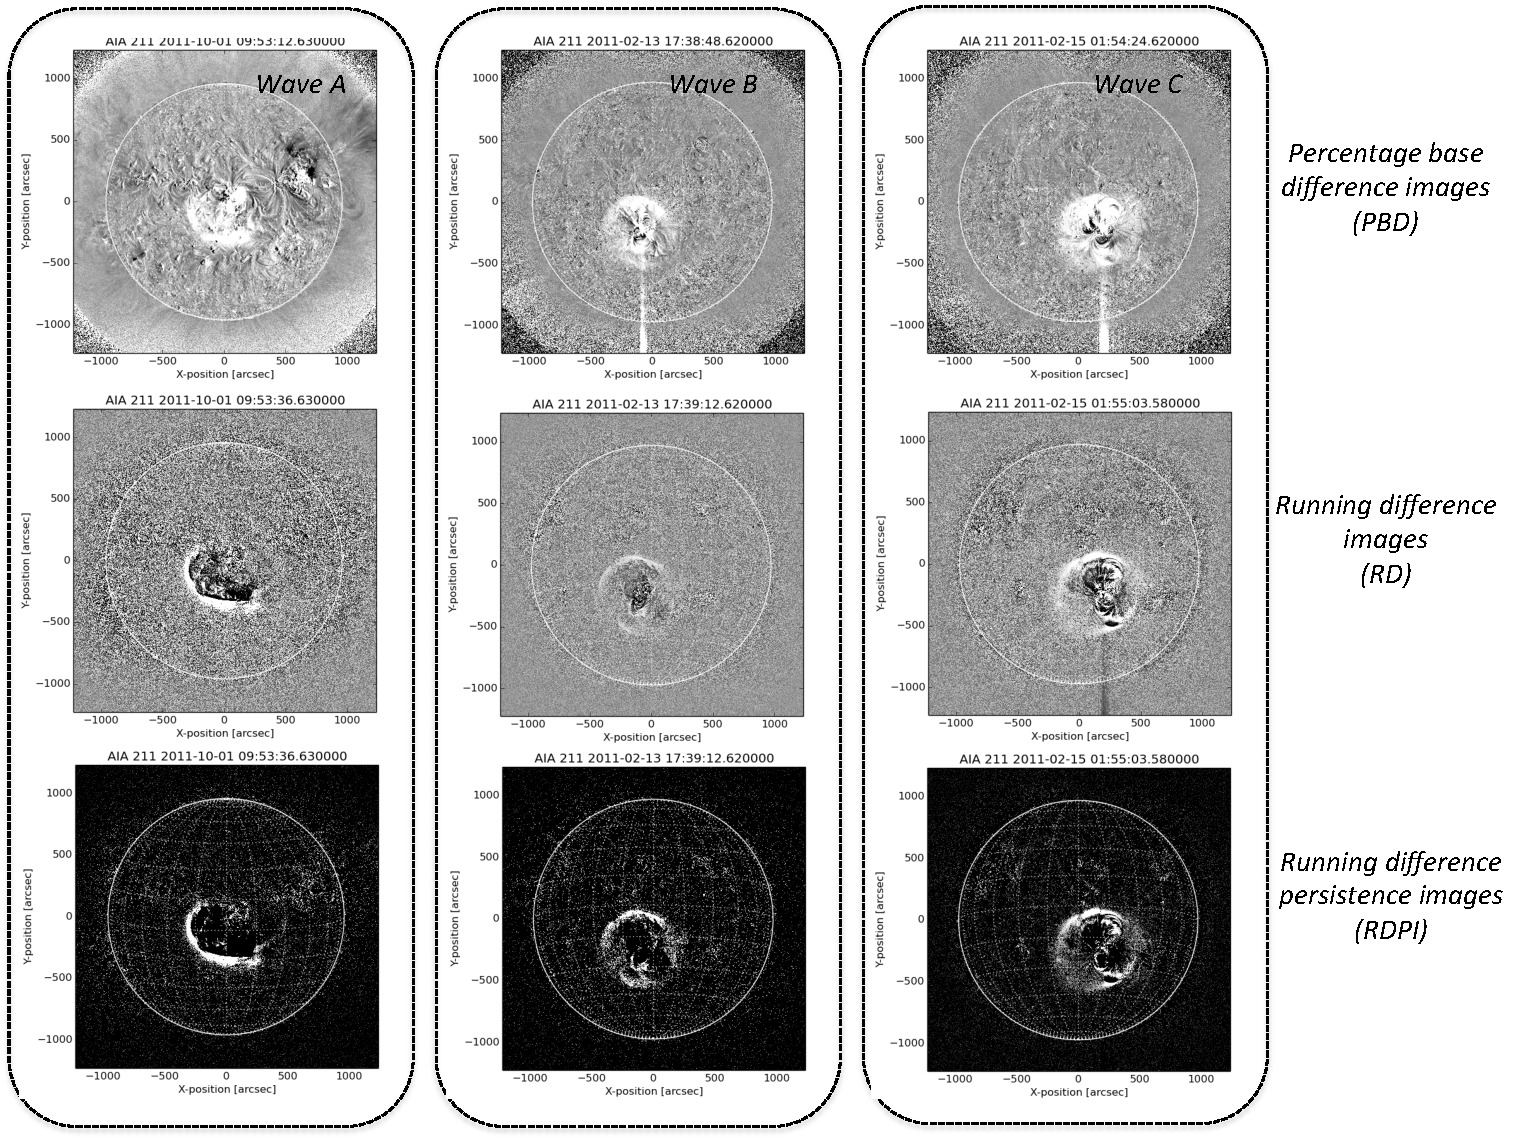
\includegraphics[width=16cm]{aware_rdpm_figure_v3.pdf}
\caption{Imaging processing techniques applied to three EUV waves, from 2011 October 1 (left column), 2011 February 13 (center column), and 2011 February 15 (right column) respectively. The top row shows percentage base difference (PBD) images of each event at a selected time, the image processing method used by the CorPITA algorithm (Long et al. 2014), while the second row shows the standard running difference (RD) images for these events (used in NEMO analysis, Podladchikova & Berghmans 2005). In the bottom row, we show that the application of running difference persistence images (RDPI) as used by AWARE is able to extract the propagating EUV wave much more cleanly. Both Wave B and Wave C were analyzed in Long et al (2014); see their Fig. 7 and 8a respectively.}
\label{rpdm_figure}
\end{center}
\end{figure}


 Figure \ref{rpdm_figure} illustrates the power of RDPIs for three example EUV wave events from 2011 October 1 (Wave A), 2011 February 13 (Wave B), and 2011 February 15 (Wave C) respectively. For each event, percentage base difference images (top row), running difference images (center row) and RDPIs (bottom row) are shown. Waves B and C from Figure \ref{rpdm_figure} were also analyzed by CorPITA in the demonstration of that algorithm by \citet{2014SoPh..289.3279L}.  The first row shows percentage base difference (PDB) images of each event, the basic image type analyzed by the CorPITA algorithm.  The second row shows running difference (RD) images, the basic image type analyzed by the NEMO algorithm.  The third row shows RDPI images, the basic image type analyzed by AWARE. Comparison with RDPIs shows that in standard RD or PBD images the wavefront is more diffuse, and much coronal structure not associated with the wavefront remains in the image. RD and PBD images also have much denser noise compared to the RDPIs of the same data; hence, separating the EUV wave from the noise is substantially easier when using RDPIs.   

Thus, the RPDI approach is the first step in the detection of EUV waves with AWARE. Subsequent image processing steps allow us to refine the detection of any propagating features. The major steps in the AWARE detection and processing algorithm are described below, and are demonstrated in Figure \ref{method_figure}.

\begin{enumerate}

\item Given a set of sequential solar EUV images (e.g. SDO/AIA or STEREO/EUVI data), create a set of persistence images, showing the brightest values obtained in each pixel in the time range 0 -> $t$

\item Perform a running difference operation on the obtained persistence images. Hence, only areas that increase in brightness from one time to the next remain (Figure \ref{method_figure}b).

\item Apply a noise reduction filter (Figure \ref{method_figure}c).  Our demonstration algorithm uses a simple two step process.  Firstly, all pixel values below a certain threshold are set to zero.  Secondly, a median filter with scale size $L$ pixels is applied.  This replaces every pixel in the image with the median value found in its neighborhood, a disk of radius $L$ pixels.

\item Apply a morphological closing \citep{2002dip..book.....G} operation to every frame in the movie (a disk with radius $L$ pixels).  This operation helps close small ‘cracks’ in structures \citep{2002dip..book.....G}.  The final image is shown in Figure \ref{method_figure}d.
\end{enumerate}

The final product is therefore a time-ordered series of images that localize the bright wavefront of the EUV wave. Figure \ref{method_figure} shows each step in this procedure, applied to two AIA 211 $\AA$ images during the EUV wave event of 2011 October 1 (Wave A in Figure \ref{rpdm_figure}). The result of the key step of generating an RDPI (Steps 1 and 2) from the two input images is illustrated in panel b). Steps 3 and 4 of the AWARE image processing method (Figure \ref{method_figure}c, d) apply some basic noise reduction and feature enhancement techniques to further refine the final images.  

\begin{figure}
\begin{center}
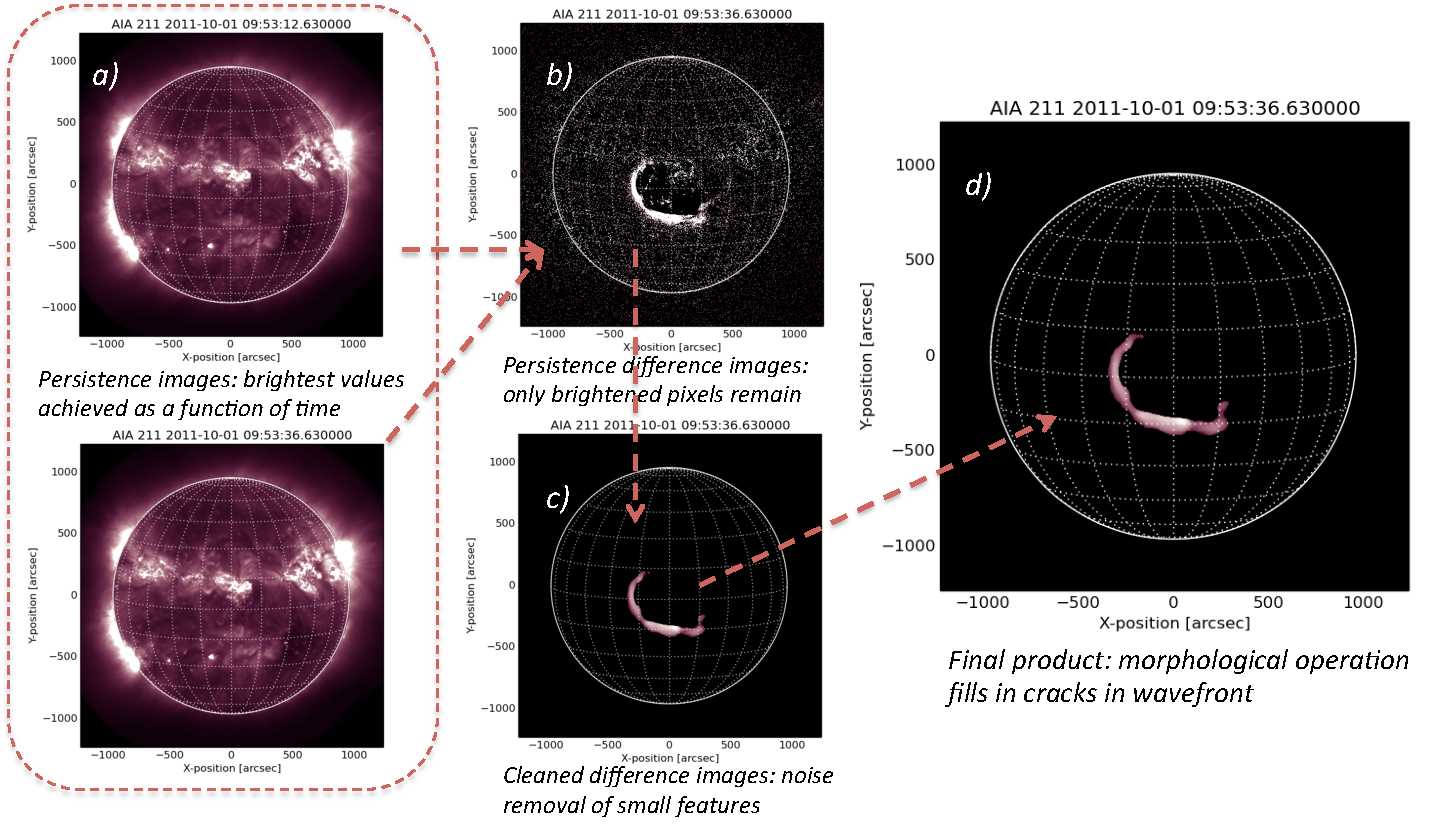
\includegraphics[width=16cm]{aware_figure4.pdf}
\caption{Example application of the AWARE image processing method. Panel a) shows two AIA 211$\AA$ images at different times during an EUV wave event. Panel b) illustrates the result of generating a running difference persistence image (RDPI) from the two input AIA images. The wavefront enhancement is evident. In panel c) a cleaning operation has been applied to the RDPI in order to remove small-scale features. Finally, in panel d) a morphological `closing operation' is applied, which has the effect of filling in small gaps in the detected wavefront \citep[e.g.][]{2002dip..book.....G}.}
\label{method_figure}
\end{center}
\end{figure}


The advantage of this approach is twofold. Firstly, we do not have to fit a complex profile to noisy data in order to locate the wavefront. Secondly, the RDPIs remove much more structure that is not associated with a propagating bright front (Fig. 2, bottom row) compared to the PBD images (Fig. 2, top-row), and therefore better isolates the wavefront, making noise-cleaning easier (Fig. 4).  NEMO \citep{2005SoPh..228..265P} uses integrals of annuli of RD images (Fig. 2, middle row) to make their detections (Sec. 2.3).  The advantage of our approach over NEMO is also twofold.  Firstly, some EUV waves do not propagate circularly (for example, wave A, Fig. 2) and therefore the annular assumption can lead to a weakened detection.  Secondly, RD images contain dimming and brightening structure unconnected with the EUV wavefront, and are noisier,  when compared to RDPIs, making isolation of the wavefront from these confounding features more difficult. The final result of the first component of AWARE is a time-series of images that may contain an EUV wave.  The second component of AWARE detects the presence of a wave, assesses its quality, and characterizes its propagation through the solar atmosphere.


\section{Results}\label{sec:results}

\subsection{Detections with simulated wave data}

\subsection{Detections with SDO/AIA image data}

Here, we illustrate the application of the AWARE algorithm to a selection of events observed by SDO/AIA.

\begin{figure}
\begin{center}
\includegraphics[width=4cm]{euvwave_contour_map_previous1.pdf}
\includegraphics[width=4cm]{euvwave_contour_map_corpita_fig7.pdf}
\includegraphics[width=4cm]{euvwave_contour_map_corpita_fig8a.pdf}
\includegraphics[width=4cm]{euvwave_contour_map_corpita_fig8e.pdf}

\includegraphics[width=4cm]{previous1.dynamics.27.pdf}
\includegraphics[width=4cm]{corpita_fig7.dynamics.2.pdf}
\includegraphics[width=4cm]{corpita_fig8a.dynamics.40.pdf}
\includegraphics[width=4cm]{corpita_fig8e.dynamics.71.pdf}
\caption{The propagation of detected EUV waves as a function of time, for a) 2011 October 1, b) 2011 February 13, c) 2011 February 15, d) 2011 February 16. For each event, a background image of the Sun is shown, while the colours represent the location of the wavefront detected by AWARE at a given time.}
\end{center}
\end{figure}






\input(5-Future_work}

\section{Conclusions}\label{sec:conclusions}

Conclusions of the work

\section{Acknowledgements}
We are grateful to the developers of SSWIDL \citep{ssw}, IPython
\citep{ipython}, SunPy \citep{mumford-proc-scipy-2013}, PyMC
\citep{pymc2010}, matplotlib \citep{Hunter:2007:matplotlib} and the
Scientific Python stack for providing data preparation, manipulation,
analysis and display packages.  LH and JI acknowledge the support of
the Solar Data Analysis Center (SDAC).



\bibliography{eitwave-paper.bib}
\bibliographystyle(swsc}

\end{linenumbers}

\end{document}
